\section{一般的概形} \label{s:1.2}

在大幅描述了仿射概形后,定义一般的概形也变得简单了。一个\textit{概形}$X$是一个拓扑空间$X$附上一个环层$\oo_X$,其中$X$被称为概形的\textit{支集}\footnote{译者注:作者后面有时会用类似``underlying space''或者``underlying set''之类的来指支集,那类词我们将翻译成“底空间”。},记作$|X|$或者$\mathrm{supp}\,X$,使得对$(|X|,\oo_X)$是\textit{局部仿射的}\index{仿射!局部}。所谓的局部仿射,就是说,$|X|$被一族开集$U_i$所覆盖,对每一个开集$U_i$存在$R_i$以及同胚$U_i\cong |\spec R_i|$使得$\oo_X|_{U_i}\cong \oo_{\spec R_i}$.

为了更好地理解这个定义,我们必须确定仿射概形的结构层的关键属性。设$X$是任意的拓扑空间,而$\oo$是它上面的一个环层,我们称偶对$(X,\oo)$为\text{赋环空间},继而我们会问,什么时候它同构于一个仿射概形$(|\spec R|,\oo_{\spec R})$. 注意到,如果$(X,\oo)$是一个仿射概形,则他将一定是概形$\spec R$.

现在令$(X,\oo)$是任意的赋环空间,以及$R=\oo(X)$. 对任意的$f\in R$,我们能定义一个集合$U_f$,其中的点$x\in X$在$f$的作用下变成了茎$\oo_x$中的可逆元。如果$(X,\oo)$是一个仿射概形,我们必须有:
\begin{compactitem}
\item[(i)] $\oo(U_f)=R[f^{-1}]$.
\end{compactitem}
然而,这个条件还不够,它甚至都没有要求$X$和$|\spec R|$之间有一个映射。为了给出这样一个映射,我们需要假设$\oo$有更多的仿射概形有的条件:
\begin{compactitem}
\item[(ii)] $\oo$的茎$\oo_x$是一个局部环。
\end{compactitem}
满足(ii)的一个赋环空间$(X,\oo)$经常被称为一个\textit{局部赋环空间}。

如果$(X,\oo)$满足(ii),那么存在一个自然映射$X\to |\spec \oo(X)|$,他将$x\in X$变成$\oo_x$的极大理想在$\oo(X)$中的原像。$(X,\oo)$要成为仿射概形的第三个要求是:
\begin{compactitem}
\item[(iii)] 映射$X\to |\spec \oo(X)|$是一个同胚。
\end{compactitem}

经过这些考虑,我们称一个偶对$(X,\oo)$是\textit{仿射的},如果它满足条件(i)--(iii). 前面给出的概形的定义现在变成了:一个偶对$(X,\oo)$是一个概形,如果他是局部仿射的。

同样,如果不产生歧义,我们将用同样的符号$X$来记概形以及其底空间$|X|$,比如在构造“令$p\in X$是一个点”中。

\begin{exe}
\begin{compactenum}[(a)]
\item 取$Z=\spec \cc[x]$,令$X$是在$|Z|$中等同两个闭点$(x)$和$(x-1)$得到的拓扑空间,以及令$\varphi:Z\to X$是自然投射。令$\oo$是$\varphi_* \oo_Z$,这是$X$上的一个环层。证明,$(X,\oo)$对每一个$f\in\oo(X)=\cc[x]$都满足前面的条件(i),但不满足条件(ii). 注意到,不存在自然映射$X\to |\spec\cc[x]|$.
\item 取$Z=\spec \cc[x,y]$,即对应于仿射平面的概形,令$X$是挖去原点的得到开子集,即$X=|Z|-\{(x,y)\}$. 令$\oo$是层$\oo_Z|_X$(即,对任意开子集$V\subset X\subset |Z|$成立$\oo(V)=\oo_Z(V)$.)证明,$\oo(X)=\cc[x,y]$,$X$, $\oo$满足条件(i)和(ii),以及自然映射$X\to |\spec\oo(X)|$是含入$X\subset |Z|$.
\end{compactenum}
\end{exe}

这里,有一些符号和术语约定如下。

一个开集$U\subset X$上的\textit{正则函数}是层$\oo_X$的在$U$上的截面。一个\textit{整体正则函数}是一个$X$上的正则函数。

结构层$\oo_X$在点$x\in X$处的茎$\oo_{X,x}$被称为$\oo_X$的\textit{局部环}。而$\oo_{X,x}$的剩余类域被记作$\kappa(x)$. 如同第 \ref{s:1.1.1} 节,$\oo_X$的一个截面能被想成一个取值于这些域$\kappa(x)$的“函数”:如果$f\in\oo_X(U)$以及$x\in U$,则$f$在点$x$处的值即$f$在复合映射
\[
	\oo_X(U)\to \oo_{X,x}\to \kappa(x)
\]
下的像。

\begin{exe}[最小的非仿射概形]
令$X$是一个拓扑开集,它只有三个点$p$, $q_1$和$q_2$. 通过令$X_1:=\{p$, $q_1\}$以及$X_2:=\{p$, $q_2\}$是开集,我们赋予了$X$一个拓扑结构(即,除了$X_1$和$X_2$外,$\varnothing$, $\{p\}$以及$X$本身是开集)。定义$X$上的一个环预层$\oo$通过置
\[
	\oo(X)=\oo(X_1)=\oo(X_2)=K[x]_{(x)},\quad \oo(\{p\})=K(x),
\]
以及限制映射$\oo(X)\to \oo(X_i)$为恒等映射,而限制映射$\oo(X_i)\to \oo(\{p\})$是显然的含入。验证这个预层是一个层以及$(X,\oo)$是一个概形。证明这不是一个仿射概形。(几何来说,这个概形$(X,\oo)$是在Exercise \ref{exe:1.44}  里的概形$X_1$中的“双重点的芽”。)
\end{exe}

\subsection{子概形} \label{s:1.2.1}

令$U$是概形$X$的一个开子集。偶对$(U,\oo_X|_U)$依然是一个层,虽然这不完全是显然的。为了检查这点,注意到,至少仿射概形的一个\textit{基本}开集依然是一个仿射概形:如果$X=\spec R$以及$U=X_f$,则$(U,\oo_X|_U)=\spec R_f$. 因为$X$中包含在$U$中的基本开集覆盖了$U$,这就证明了$(U,\oo_X|_U)$由仿射概形所覆盖,此即所需。在上述概形结构下,概形的一个开子集被称为概形的一个\textit{开子概形}。

闭子概形的定义更加复杂,指定$X$的一个闭子集是不够的,因为上面的层结构不能顺道定义出来。

首先考虑一个仿射概形$X=\spec R$. 对环$R$的任意理想$I$,我们将闭子集$V(I)\subset X$与仿射概形$Y=\spec R/I$等同。这个等同的成立是因为$R/I$的素理想正好就是$R$中那些素理想模去$I$得到的,因此拓扑空间$|\spec R/I|$是典范同构于闭子集$V(I)\subset X$. 我们将$X$的一个\textit{闭子概形}定义为$R$的一个商环的谱(于是按定义,$X$的闭子概形一一对应于环$R$中的一个理想)。

进而,我们可以定义给定概形$X=\spec R$的闭子概形上的那些常见的操作以及闭子概形间的关系。因此,对$X$闭子概形$Y=\spec R/I$和闭子概形$Z=\spec R/J$,如果$Z$是一个$Y$的闭子概形,即$J\supset I$,则称$Y$\textit{包含}$Z$. 这可以推出$V(J)\subset V(I)$,但是反过来并不对。

\begin{exe}\label{exe:1.26}
	Exercise \ref{exe:1.20} 中的概形$X_1$, $X_2$, $X_3$都能被看作$\spec \cc[x]$的闭子概形。证明
	\[
	X_1\subset X_3\quad \text{以及}\quad X_2\subset X_3,
	\]
	但是没有其他包含$X_i\subset X_j$成立,尽管$X_2$和$X_3$的底空间相同,且都包含$X_1$的底空间。
\end{exe}

两个闭子概形$\spec R/I$和$\spec R/J$的\textit{并}被定义为$\spec R/(I\cap J)$,它们的\textit{交}被定义为$\spec R/(I+J)$. 注意,这些包含、相交与并的概念\textit{并不}满足它们在集合中的对应概念的那些寻常性质:比如,我们将在第 \pageref{p:69} 页上发现这样一个例子,一个概形的闭子概形们$X$, $Y$, $Z$满足$X\cup Y=X\cup Z$以及$X\cap Y=X\cap Z$但$Y\neq Z$.

现在我们要把闭子概形的概念拓展到一般的概形$X$上。为此,第一步需是用一个层代替仿射概形$X=\spec R$中伴随于闭子概形$Y$的理想$I\subset R$,现表述如下。定义$Y$\textit{在}$X$\textit{中的理想层} $\scr{J}=\scr{J}_{Y/X}$为$\oo_X$的一个理想层,它在每一个$X$的基本开集$V=X_f$上给出$\scr{J}(X_f)=I R_f$. 现在可以将$Y=\spec R/I$的结构层$\oo_Y$(更准确地说,是在含入映射$j:|Y|\hookrightarrow |X|$下的前推$j_{*}\oo_Y$)与商层$\oo_X/\scr{J}$等同起来。(请自行检验这个等同。)理想层$\scr{J}$将作为限制映射$\oo_X\to j_*\oo_Y$的核被还原出来。

这儿有一个不易察觉的点需要指出:并非所有$\oo_X$的理想层都可以从$R$的理想得到。比如,在Example \ref{exa:1.22} 中考虑的$R=K[x]_{(x)}$,我们可以如下定义一个理想层
\[
	\scr{J}(X)=0,\quad \text{以及对$U=\{(0)\}$, }\scr{J}(U)=\oo_X(U).
\]
但是如果$\scr{J}$来自于$R$的一个理想,我们应该有
\[
	\scr{J}(U)=\scr J (X)_x = \scr J (X) K(x),
\]
于是$\scr J$并不是来自于$R$的某个理想。在前面的闭子概形的定义中,我们将只关注来自于$R$的理想的理想层。这样一个理论中的层显然需要一个名字:它们被称为\textit{拟凝聚}理想层。(对这样一个基础而简单的对象,看上去这是一个缺乏启发性的名字,但它却坚实扎根于各个文献中。它来自于Noether环的素谱上的层对应于具有被称为凝聚性的性质的有限生成模\footnote{译者注:凝聚模是一个有限生成模,它的任意有限生成子模都需要是有限表示的。}的事实;因此,我们自然会说来自于有限生成模的层是\textit{凝聚的},而来自于任意模的层是\textit{拟凝聚的}。)

更一般地,一个任意概形$X$上的\textit{拟凝聚理想层}$\scr J \subset \oo_X$是一个理想层$\scr J$使得,对每一个仿射开集$U\subset X$,限制$\scr J|_U$是一个$U$上拟凝聚理想层。

现在,我们已准备定义闭子概形,这是一个局部看上去是一个仿射概形的闭子概形的东西:

\begin{defi}\label{defi:1.27}
	如果$X$是任意的概形,则$X$的\textit{闭子概形}$Y$是一个闭子空间$|Y|\subset |X|$连同一个环层$\oo_Y$,这个环层是结构层$\oo_X$模去一个拟凝聚理想层$\scr J$得到的商层,并且$Y$与任意仿射开集$U\subset X$的交是一个关联于理想$\scr J(U)$的闭子概形。

	设$V\subset X$是任意的开集,对正则函数$f\in \oo_X(V)$,如果$f\in \scr J(V)$,则我们称$f$\textit{在}$Y$\textit{上为零}。
\end{defi}

实际上,$|Y|$由$\scr J$唯一确定\footnote{译者注:这里,包括上面的定义,作者表述地不算很清楚。首先,$\oo_Y=\oo_X/\scr J$是一个$X$上的层,其所有茎非零的点(一般被称为支集)构成了$X$的一个闭子集$Y$,然后我们可以将$\oo_Y$限制在$Y$上得到概形$(Y,\oo_Y)$. 这里所谓的限制可以这样理解,任取$Y$中的开集$V$,都存在$X$中的开集$U$使得$V=U\cap Y$,然后定义$\oo_Y(V)=(\oo_X/\scr J)(U)$. 不难证明,如果$Y$是闭集,则这个定义与$U$的选取无关。

为证明$\oo_Y$的支集$Y$是闭的,注意到给定一个开覆盖$\{U_i\}$,一个集合$V$是闭集,当且仅当$U_i\cap V$在每一个$U_i$中是闭集,所以我们只需在每一个仿射开集$U$中考察。由于$Y\cap U$此时是关联于$\scr J(U)$的子概形,则$(\oo_X/\scr J)|_U$在$\spec(\oo_X(U))$上的支集此时就是包含$\scr J(U)$的素理想的全体,是闭集$V(\scr J(U))$.},因此$X$的闭子概形一一对应于拟凝聚理想层$\scr J\subset \oo_X$.

拟凝聚的概念也会出现在一些更广义的上下文中。我们类似定义$X$上的\textit{拟凝聚层}$\scr F$为一个$\oo_X$-模层(即对每一个$U$,$\scr F(U)$是一个$\oo_X(U)$-模),对任意仿射开集$U$以及基本开集$U_f\subset U$,$\oo_X(U_f)=\oo_X(U)_f$-模$\scr F(U_f)$可以由$\scr F(U)$通过局部化$f$得到,更准确地说,限制映射$\scr F(U)\to \scr F(U_f)$在局部化$f$后是一个同构\footnote{译者注:怎么说呢,我个人感觉作者在这里写得也乱七八糟的。这段看不懂可以参考EGA I的定理1.4.1. }。$\scr F$被称为\textit{凝聚的},如果每一个$\scr F(U)$都是有限生成的。(有时会在更具限制的时候使用“凝聚”这个词汇,但是当$X$被有限个Noether环的谱所覆盖的时候,这俩意思是相同的,而这一种情况也是主要的兴趣所在)也许有些人会没那么正式地说,拟凝聚层是那些模层,它们限制在仿射开集上是对应的环上的模(如果是凝聚层的情况就是有限生成模)。这是概形语境下关于环上的模的正确对应,在大多数情况下,我们可以把它们简单想做模。

\begin{exe}\label{exe:1.28}
为检查一个理想层(或任意模层)是拟凝聚的(或者说是凝聚的),只要检查在给定$X$的仿射开覆盖的每个仿射开集上检查即可。
\end{exe}

仿射概形$X$的最重要闭子概形之一就是$X_{\text{red}}$,$X$的\text{约态概形}。这可以直接由$X_{\text{red}}=\spec R_{\text{red}}$,其中$R_\text{red}$是$R$磨去它的\textit{幂零根},即模去$R$所有幂零元构成的理想。回忆,$R$的幂零根等于$R$的所有素理想的交(实际上,是所有极小素理想的交)。因此,$|X|$和$|X_\text{red}|$作为拓扑空间是相同的。

\begin{exe}\label{exe:1.29}
$X_\text{red}$同样可以由拓扑空间$|X|$连同结构层$\oo_{X_\text{red}}$定义,对每一个开集$U\subset X$,$\oo_{X_\text{red}}(U)$就是环$\oo_X(u)$模去其幂零根。
\end{exe}

为了将这个概念推广到全局,我们对任意概形$X$可以定义一个理想层$\scr N\subset \oo_X$,称为\textit{幂零根},它在每一个开集$U$上就是$\oo_X(U)$的幂零根。因为幂零根的构造与局部环可以交换,$\scr N$是一个拟凝聚理想层。这个拟凝聚理想层对应的闭子概形被称为$X$的\textit{约态概形},记作$X_\text{red}$.

\textit{不可约性}是概形另一个可能的性质,尽管是这个名字,但它与概形是否约态无关。一个概形$X$是\textit{不可约的}如果$|X|$不能写作两个真闭子集的并。关于约态和不可约概形,这里有些简单但重要的附注。

\begin{exe}
	一个概形是不可约的当且仅当每一个开子集都是稠密的。
\end{exe}

\begin{exe}
	一个仿射概形$X=\spec R$是约态且不可约的,当且仅当$R$是一个整环。$X$是不可约的当且仅当$R$只有一个极小素理想,或者等价地,$R$的幂零根是一个素理想。
\end{exe}

\begin{exe}
	一个概形$X$是约态的,当且仅当每一个$X$的仿射开子概形是约态的,当且仅当,对每一个闭点$p\in X$,局部环$\oo_{X,p}$是约态的。(一个环被称为约态的,如果他唯一的幂零元是$0$.)
\end{exe}

\begin{exe}
	如何定义两个概形的不交并?证明两个仿射概形$\spec R$和$\spec S$的不交并应当等同于概形$\spec R\times S$.
\end{exe}

\begin{exe}
	一个任意的概形$X$是不可约的,当且仅当它每一个仿射开子集是不可约的。如果它还是连通的(即指其拓扑空间$|X|$是连通的),于是它是不可约的当且仅当每一个$\oo_X$的局部环都只有一个唯一的极小素理想。
\end{exe}

我们现在已经引入了概形$X$的开子概形与闭子概形的概念。更进一步,一个$X$的\textit{局部闭子概形}的定义是直接的:它是一个$X$的开子概形的闭子概形。这是本书中我们可能考虑的最一般概念,于是,当我们只说$X$的一个子概形,没有修饰语的时候,我们就是在说局部闭子概形。

\begin{exe}
令$X$是一个任意的概形,而$Y$, $Z$是它的闭子概形。解释$Y$包含于$Z$中的意思是什么。同样,如果$Y$, $Z$只是局部闭子概形,则$Y$包含于$Z$中的意思是什么。
\end{exe}

给定$X$的一个局部闭的子概形$Z\subset X$,我们定义$Z$的\textit{闭包}$\overline{Z}$为$X$中包含$Z$的最小的闭子概形,即,$X$所有包含$Z$的闭子概形的交。等价地,如果$Z$是一个开子概形$U\subset X$的闭子概形,闭包$\overline{Z}$是一个$X$的由限制在$U$上后在$Z$上为零的正则函数的理想层定义的闭子概形\footnote{译者注:原文读起来相当拗口,这里解释一下。首先,在$U$上,$Z$是一个闭子概形,对应有一个$U$上的拟凝聚理想层$\scr J$. 这里正则函数$f$限制在$U$上后在$Z$上为零的意思就是$f|_U\in \scr J(U)$.}。

\subsection{一点处的局部环} \label{s:1.2.2}

在环理论中,Noether性是非常基本的,而它在概形理论中的拓展也是同样基本的:我们称一个概形是Noether的,如果它可以被有限个仿射开子概形覆盖,其中每个仿射开子概形都是某个Noether环的谱。就像通常的情况,我们可以检查这个性质与选取的覆盖是无关的。

在概形$X$的一点$x$处的芽有一个自然的定义,它是所有包含这点的开子概形的交。这体现为$X$在点$x$处的\textit{局部环},之前定义为
\[
	\oo_{X,x}:={\varinjlim}_{x\in U}\oo_X(U).
\]
它的极大理想$\mm_{X,x}$是所有在$x$处为零的截面的集合。这个局部环是一个简单的对象:为计算它(特别地,展示它是一个局部环,极大理想就是我们给出的极大理想),我们先用一个$x$的仿射开集来代替$X$,于是假设$X=\spec R$以及$x=[\pp]$. 我们接着把直极限中的开集取作基本开集$\spec R_f$使得$f(x)\neq 0$,即$f\not\in \pp$. 于是
\[
	\oo_{X,x}:={\varinjlim}_{f\not\in \pp}R_f=R_{\pp}
\]
以及
\[
	\mm_{X,x}:={\varinjlim}_{f\not\in \pp}\pp R_f=\pp R_{\pp},
\]
就是$R$在$\pp$处的局部化。我们可以认为$X$在$x$处的芽是$\spec \oo_{X,x}$,这样的概形我们将在下一章里面研究。

概形在一点处的局部环的概念在整个概形理论里面是十分关键的。我们下面会给出一些例证,来展示如何使用局部环定义一些几何概念。令$X$是一个概形。

\vspace{0.5em}
(1) \textit{$X$在一点$x\in X$处的维数},记作$\dim(X,x)$,是局部环$\oo_{X,x}$的(Krull)维数,即$\oo_{X,x}$中素理想链的长度的上确界。(链的长度是严格包含的个数。)$X$的\textit{维数},记作$\dim X$,是这些局部维数的上确界。

\begin{exe}
	零维仿射概形的底空间是有限的。
\end{exe}

(2) $X$在$x$处的\textit{Zariski余切空间}是$\mm_{X,x}/\mm_{X,x}^2$,看作剩余类域$\kappa(x)=\oo_{X,x}/\mm_{X,x}$上的矢量空间。这个矢量空间的对偶空间被称为$x$处的\textit{Zariski切空间}。

为理解这个定义,首先考虑一个非奇异的复代数簇$X$. 此时,$X$在点$p$处的切空间的定义是明确的:他是它这点的解析函数芽映到$\cc$的导子的矢量空间。如果$\mm_{X,p}$是在点$p$处为零的正则函数构成的理想,那么这样一个导子就将诱导出一个$\cc$-线性映射$\mm_{X,p}/\mm_{X,p}^2\to \cc$,于是切空间可以通过这种方式等同为$\Hom_\cc(\mm_{X,p}/\mm_{X,p}^2,\cc)=(\mm_{X,p}/\mm_{X,p}^2)^*$. 见Eisenbud [1995, Ch. 16]. Zariski洞察到,后一个矢量空间是任意簇上的不管光滑还是奇异的点上的切空间的正确类比,Grothendieck随后将这个想法应用到了概形上,就像上面给出的定义。我们将在第 \ref{chap:6} 章以一种新的视角回到这个构造。

\begin{exe}
如果$K$是一个域,则概形$\spec K[x_1$, $\dots$, $x_n]$在点$[(x_1$, $\dots$, $x_n)]$处的Zariski切空间是$n$维的。
\end{exe}

(3) $X$被称为在点$x\in X$处\textit{非奇异}(或\textit{正则})如果$X$在$x$处的Zariski切空间的维数等于$\dim(X,x)$,否则,Zariski切空间的维数一定是会更大,此时我们称$X$在$x$处奇异。在我们最感兴趣的情况中,$X$是Noether的,此时$X$在$x$处非奇异当且仅当局部环$\oo_{X,x}$是一个正则局部环。历史上,这个基础的概念代表了几何代数化的重要一步。他被Zariski在其经典论文[1947]中所采用(值得注意,这是在Krull引入正则局部环的概念来拓展多项式环性质的几年后,是少数几个代数学家在基础几何概念上击败几何学家的例子之一)。

\begin{exe}
一个零维Noether概形是非奇异的,当且仅当他是约态点的并。
\end{exe}

\subsection{态射} \label{s:1.2.3}

下面定义概形的态射。在经典理论中,仿射簇之间的正则映射由其坐标环之间的相反方向的映射给出。这个对应使得两类对象,仿射簇之间的正则映射以及其坐标代数之间的代数同态,是等价的。下面给出的定义拓展了这点:我们将看到仿射概形之间的映射仅由对应的环之间的(方向相反的)映射给出。

在用环之间的映射给出了仿射概形之间映射的简单描述后,我们可能想要将概形间的态射定义为某种“局部是仿射概形之间的态射”的东西。我们可以尝试去那么做,这将给出正确的答案,但这也将导致一个麻烦的问题,即需要检查这个定义是与仿射覆盖的选取无关的。因此,我们在下面给出一个与仿射覆盖选取无关的定义。尽管第一次看到它的时候可能觉得它有些复杂,但在实践中,这是方便的。同时,这个定义也可以应用到所有的“局部赋环空间”上,这是一个拓扑空间连同上面一个环层,层上每条茎都是局部环。

为了理解这个定义背后的动机,再一次考虑可微流形的例子。一个可微流形之间的连续函数$\psi:M\to N$是可微的,当且仅当,对每一个开集$U\subset N$上的可微函数$f$,拉回$\psi^\# f:=f\circ \psi$是一个在$\psi^{-1}U\subset M$上的可微函数。我们很容易用概形的语言来表述这点。任意连续函数$\psi:M\to N$诱导了$N$上的层之间的映射
\[
	\psi^\#:\mathscr C(N)\to \psi_*\mathscr C(M),
\]
他将开集$U\subset N$上的连续函数$f\in \mathscr C(N)(U)$变成了拉回$f\circ \psi\in \mathscr C(M)(\psi^{-1}U)=(\psi_*\mathscr C(M))(U)$. 在这些术语下,一个可微映射$\psi:M\to N$可以定义为一个连续映射$\psi:M\to N$使得诱导的映射$\psi^\#$将子层$\mathscr C\infty(N)\subset \mathscr C(N)$映到子层$\psi_*\mathscr C\infty(M)\subset \psi_*\mathscr C(M)$. 即,我们要求存在交换图
\[
	\xymatrix{
	\mathscr C(N)\ar[r]^{\psi^\#}&\psi_*\mathscr C(M)\\
	\mathscr C^\infty(N)\ar[r]^{\psi^\#}\ar@{^{(}->}[u]&\psi_*\mathscr C^\infty(M)\ar@{^{(}->}[u]
	}
\]

我们将应用这个思想到概形上。这里的区别是,概形$X$的结构层$\oo_X$不是一个给定的$X$上的函数层的子层。因此,为了给出概形之间的映射,我们必须\textit{同时}给定底空间之间的连续映射$\psi:X\to Y$以及拉回
\[
	\psi^\#:\oo_X\to\psi_*\oo_Y.
\]
当然,$\psi^\#$和$\psi$必须满足一些相容性条件。可在给定它们的时候会遇到如下问题,结构层$\oo_Y$的截面并不在某一个固定的域中取值,它在域$\kappa(q)$上取值,会随着$q\in Y$而改变。特别地,要求$f\in\oo_Y(U)$在点$q\in U\subset Y$上的值等于$\psi^\# f\in \psi_*\oo_X(U)=\oo_X(\psi^{-1}U)$在一个点$p\in \psi^{-1}q\subset \psi^{-1}U\subset X$上的值变得毫无意义(当像在可微函数上那样定义$\psi^\#$时,这是有效的),因为这些“值”取在不同的域中。但要求$f$在点$q$为零当且仅当$\psi^\# f$在点$q$为零是有意义的,而这正是所需要的。进而我们给出下面的定义。

\begin{defi}
一个概形$X$和$Y$之间的\textit{态射},或\textit{映射}是一个有序对$(\psi,\psi^\#)$,其中$\psi:X\to Y$是一个底空间之间的连续映射而
\[
	\psi^\#:\oo_Y\to \psi_*\oo_X
\]
是一个$Y$上的层之间的映射,满足对任意的$p\in X$以及$Y$中$q=\psi(p)$的任意邻域$U$,一个截面$f\in\oo_Y(U)$在点$q$处为零当且仅当$\psi_*\oo_X(U)=\oo_X(\psi^{-1}U)$中的截面$\psi^\# f$在$p$处为零。
\end{defi}

最后一个条件可以用局部环$\oo_{X,p}$和$\oo_{Y,q}$很漂亮地重新表述如下。层之间的任意映射$\psi^\#:\oo_Y\to \psi_* \oo_X$取直极限后诱导了映射
\[
	\oo_{Y,q}={\varinjlim}_{q\in U\subset Y}\oo_Y(U)\to {\varinjlim}_{q\in U\subset Y}\oo_X(\psi^{-1}U),
\]
后一个环自然地映射到直极限
\[
	{\varinjlim}_{p\in V\subset X}\oo_X(V),
\]
其中$V$跑遍所有包含$p$的开集,此即$\oo_{X,p}$. 因此,$\psi^\#$诱导了局部环之间的一个映射$\oo_{Y,q}\to \oo_{X,p}$. 称一个截面$f\in \oo_Y(U)$在点$q$处为零,当且仅当$\psi^\# f\in \psi_*\oo_X(U)=\oo_X(\psi^{-1}U)$在点$p$处为零,就是在说映射$\oo_{Y,q}\to \oo_{X,p}$将极大理想$\mm_{Y,q}$映射到了$\mm_{X,p}$,换而言之,这是局部环之间的\textit{局部同态}。

如前所言,一个仿射概形之间的态射
\[
	\psi:X=\spec S\to\spec R=Y
\]
与环同态$\varphi:R\to S$无异。下面是精确的结果,还略带改进,描述了从任意概形到仿射概形的映射。

\begin{thm}\label{thm:1.40}
对任意的概形$X$以及任意的环$R$,态射
\[
	(\psi,\psi^\#):X\to \spec R
\]
一一对应于环同态
\[
	\varphi:R\to \oo_X(X)
\]
通过
\[
	\varphi=\psi^\#(\spec R):R=\oo_{\spec R}(\spec R)\to \psi_*(\oo_X)(\spec R)=\oo_X(X).
\]
\end{thm}

\begin{proof}
我们下面描述反过来的对应,即对一个环同态,找一个概形态射。令$Y=\spec R$以及$\varphi:R\to \oo_X(X)$是交换环同态。设$p\in |X|$是一个点,则极大理想在复合$R\to \oo_X(X)\to \oo_{X,p}$下的原像是一个素理想,于是$\varphi$诱导了集合间的映射
\[
	\psi:|X|\to |Y|,
\]
不难检验在Zariski拓扑下这是连续的。接着,对每一个基本开集$U=\spec R_f\subset Y$,定义映射$\psi^\#:R_f=\oo_Y(U)\to (\psi_*\oo_X)(U)$是由局部化$\psi$得到的复合
\[
	R_f\to \oo_X(X)_{\varphi(f)}\to \oo_X(\psi^{-1}U).
\]
从Proposition \ref{pro:1.12}(ii),我们只要定义层之间的态射即可。进一步局部化,我们看到如果$\psi(p)=q$,则$\psi^\#$定义了一个局部环之间的局部同态$R_q\to \oo_{X,p}$,因此$(\psi,\psi^\#)$是一个概形间的态射。很清楚,诱导映射满足
\[
	\psi^\#(Y)=\varphi,
\]
于是这个构造就是命题中对应的逆。
\end{proof}

当然,这个结果告诉我们,特别地,所有仿射概形范畴中的信息其实已经存在于交换环范畴中。

\begin{coro}\label{coro:1.41}
	仿射概形范畴等价于箭头倒过来的含幺交换环范畴,即所谓的对偶范畴。
\end{coro}

\begin{exe}\label{exe:1.42}
	\begin{compactenum}[(a)]
	\item 使用这个证明,从任意概形到$\spec \zz$存在且只存在一个映射。以范畴论的语言,这就是在说$\spec \zz$是概形范畴的\idx{终对象}。
	\item 证明,单点集是集合范畴的终对象。
	\end{compactenum}
\end{exe}

比如,$X=\spec R$的每个点$[\pp]$对应有个概形$\spec \kappa(\pp)$,以及一个由如下复合环映射
\[
	R\to R_\pp\to R_\pp/\pp_\pp=\kappa(\pp)
\]
定义的到$X$的自然映射。当然,含入使得$[p]$是一个闭子概形当且仅当$\pp$是$R$的一个极大理想(一般地,$[\pp]$是一个闭子概形的无限开子概形的交)。

如果$\psi:Y\to X$是一个仿射概形间的态射,$X=\spec R$和$Y=\spec T$,$X'$是由$R$的理想$I$定义的$X$的闭子概形,于是,我们定义$\psi$在$X'$上的原像(有时,为了强调这个构造,我们会说“概形意义上的原像”)$\psi^{-1}X'$为$Y$中由$T$的理想$\varphi(I)T$定义的闭子概形。如果$X'$是$X$的一个闭点$p$,我们称$\psi^{-1}p$是$X'$上的\textit{纤维}。(我们马上就会看到如何在任意点上定义纤维。)原像的底空间就是集合意义上的原像,然而原像的概形结构将给出一个巧妙且实用的“正确的重数”的概念来计数原像中的点。最简单的经典例子以后会在Exercise \ref{exe:2.2} 给出,这里我们给出另外两个。

\begin{exe}\label{exe:1.43}
\begin{compactenum}[(a)]
\item 令$\varphi:X\to Y$是如下展示的仿射概形之间的映射
\begin{center}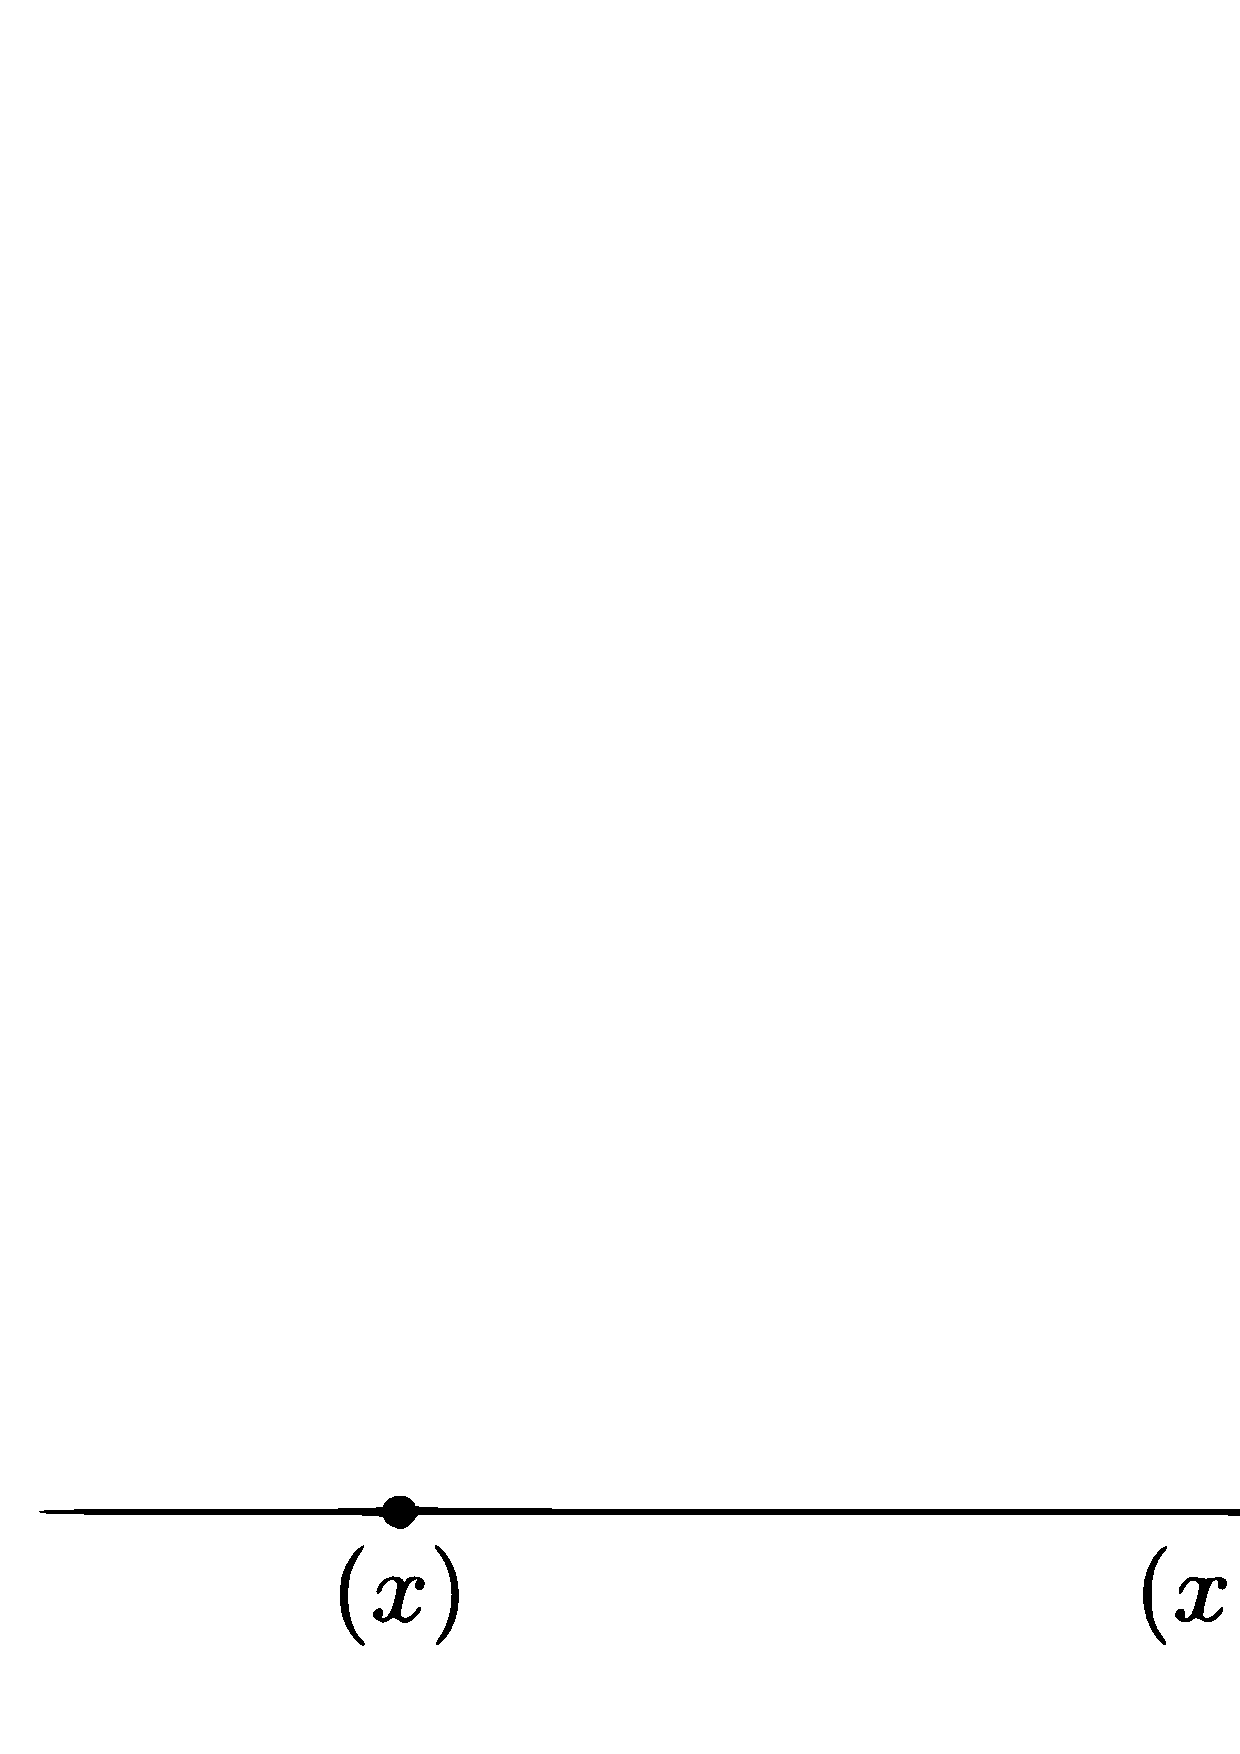
\includegraphics[scale=\scale,bb=0 0 257 227]{\PICDIR/1.png}\end{center}
即,$X=\spec K[x,u]/(xu)$是两条在点$p=(x,u)$处相交的直线的交,而$Y=\spec K[t]$是一条直线,映射在每一条$X$的直线上都是同构。比如,它可以由环同态
\[
	\begin{array}{rcl}
	K[t]&\to &K[x,u]/(xu),\\
	t&\mapsto&x+u.
	\end{array}
\]
给出。证明,若$a\neq 0$,则点$q_a=(t-a)$处的纤维是概形$\spec(K\times K)$,它包含两个不同的点。然而,点$q_0$处的纤维包含双重点$p$,同构于$\spec K[x]/(x^2)$. 代数$K[x]/(x^2)$(作为$K$-矢量空间)是二维的这点反应了映射在$p$处局部的结构。
\item 令$\varphi:X\to Y$是如下展示的仿射概形之间的映射
\begin{center}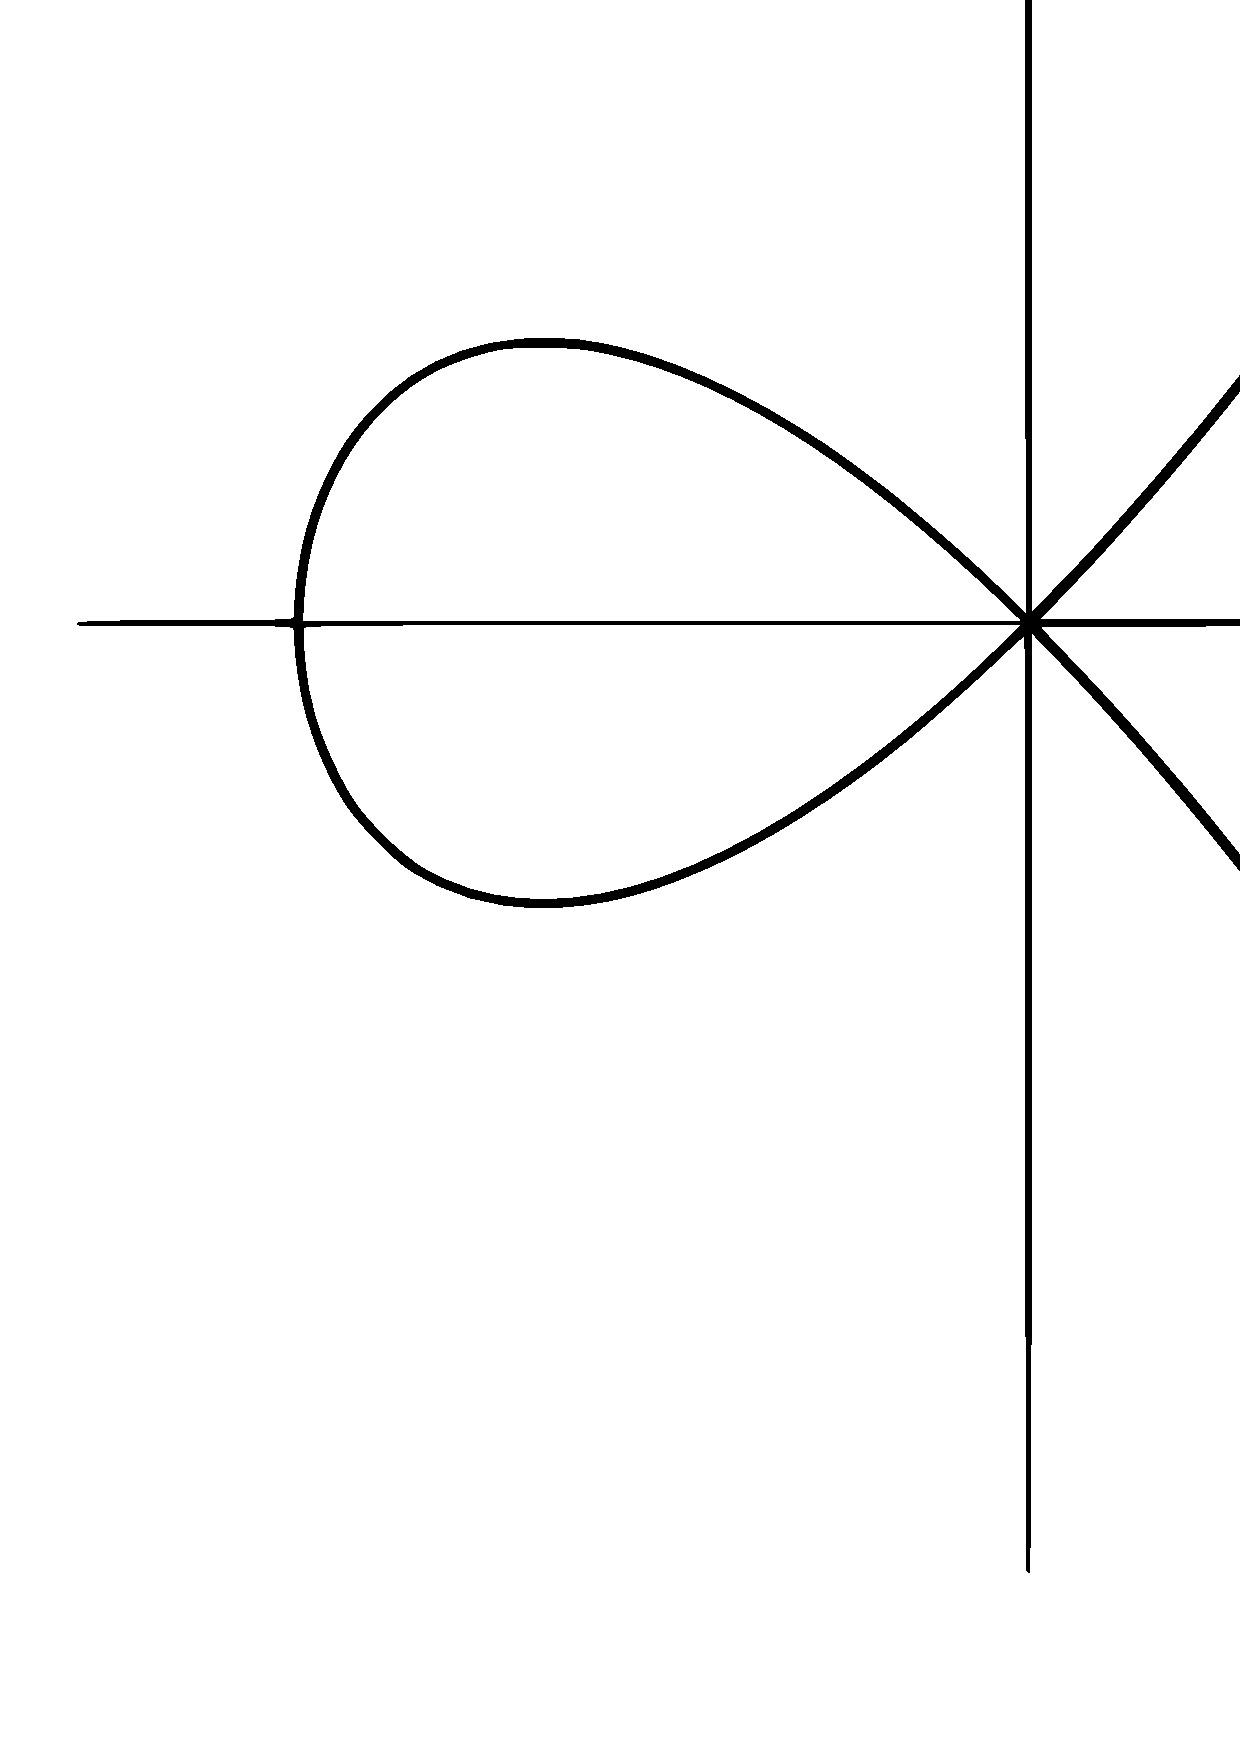
\includegraphics[scale=\scale,bb=0 0 320 352]{\PICDIR/2.png}\end{center}
即,$X=\spec K[x,y,u,v]/((x,y)\cap (u,v))$是两个4-空间的平面,它们交于同一点$p=(x,y,u,v)$,而$Y=\spec K[s,t]$是一个平面,映射在每一个$X$的平面上都是同构。比如,它可以由环同态
\[
	\begin{array}{rcl}
	K[s,t]&\to &K[x,y,u,v],\\
	t&\mapsto&x+u,\\
	s&\mapsto&y+v.
	\end{array}
\]
证明,如果$a$或者$b$不全为零,则
\[
	q_{a,b}=(s-a,t-b)
\]
的纤维是$\spec(K\times K)$,包含两个不同的点。然而,$q_{0,0}$处的纤维包含了“双重点”$p$,同构于
\[
	\spec K[x,y]/(x^2,xy,y^2).
\]
代数$K[x,y]/(x^2,xy,y^2)$在一个$K$上的三维矢量空间这点反应了关于簇$X$的一个深刻事实(它不是“局部Cohen-Macaulay的”)。这个例子将在第 \ref{s:2.3.4} 小节以平坦性的观点再次捡起。
\end{compactenum}
\end{exe}

\subsection{黏合构造} \label{s:1.2.4}

使用态射的概念,我们可以通过将简单的概形沿着开集等同起来构造更复杂的概形(比如非仿射概形)。这个基本的操作被称为\textit{黏合构造}。

假设我们给定了一族概形$\{X_\alpha\}_I$,对$I$中每一个$\beta\neq \alpha$,我们给一个$X_\alpha$的开集$X_{\alpha\beta}$. 同样假设,我们已经给定了一族概形的同构
\[
	\psi_{\alpha\beta}:X_{\alpha\beta}\to X_{\beta\alpha}\quad \text{对$I$中的每对$\alpha\neq \beta$},
\]
满足$\psi_{\alpha\beta}=\psi_{\beta\alpha}^{-1}$对所有$\alpha$和$\beta$都成立,且
\[
	\psi_{\alpha\beta}(X_{\alpha\beta}\cap X_{\alpha\gamma})=X_{\beta\alpha}\cap X_{\beta\gamma}\quad \text{对所有$\alpha$, $\beta$, $\gamma$都成立,}
\]
还有相容性条件
\[
	\psi_{\beta\gamma}\circ \psi_{\alpha\beta}|_{(X_{\alpha\beta}\cap X_{\alpha\gamma})}=\psi_{\alpha\gamma}|_{(X_{\alpha\beta}\cap X_{\alpha\gamma})}.
\]
在那种情况下,我们可以以一种显然的方式将$X_\alpha$沿着$\psi_{\alpha\beta}$黏合起来定义一个概形,即,存在一个(唯一的)概形$X$,它由同构于$X_\alpha$的开子概形所覆盖,并且交$X_\alpha\cap X_\beta\subset X$上的恒等映射对应于同构$\psi_{\alpha\beta}$.

这个构造比如能用来从仿射概形构造出射影概形。在环面簇(toric variety)理论中有另外的应用,比如见Kempf等[1973].

在这些和几乎所有的应用中,我们实际上不需要明确地给出映射$\psi_{\alpha\beta}$:我们实际上是给出了一个拓扑空间$|X|$以及一族开集$|X_\alpha|$,每一个开集上都有一个仿射概形结构,即有一个结构层$\oo_{X_\alpha}$,此时$\oo_{X_\alpha}(X_\alpha\cap X_\beta)$\textit{自然地}等同于$\oo_{X_\beta}(X_\alpha\cap X_\beta)$. 比方说,它们可能同时作为一个固定集合的子集给出。在这种情况下,Corollary \ref{coro:1.14} 的条件是立即满足的,进而$X$上存在唯一确定的层$\oo_X$延拓了所有的$\oo_{X_\alpha}$. 于是,偶对$(|X|,\oo_X)$是一个概形。

也许最简单的例子是任意概形$S$上的\textit{仿射空间}$\mathbb{A}^n_S$. 首先,对任意仿射概形$X=\spec R$,我们定义$X$\text{上的仿射$n$-空间}为$\spec R[x_1$, $\dots$, $x_n]$,记作$\mathbb{A}_X^n$或$\mathbb{A}_R^n$. (仿射空间及其子概形的几何将在第 \ref{chap:2} 章重新捡起。)接着,注意到任意的仿射概形态射$X\to Y$诱导了自然的映射$\mathbb{A}_X^n\to \mathbb{A}_Y^n$. 于是,我们可以如下利用黏合构造:如果$S$是任意的概形,$U_\alpha=\spec R_\alpha$是其开覆盖,我们定义\textit{$S$上仿射空间$\mathbb{A}_S^n$}为仿射空间$\mathbb{A}_{U_\alpha}^n$沿着$U_\alpha\cap U_\beta$上的恒等映射黏起来得到的概形。

我们后面将看到另外两种在任意概形$S$定义仿射空间$\mathbb{A}_S^n$的方法,见Exercise \ref{exe:1.47} 和\ref{exe:1.54}.

下面的习题展示了一些黏合构造的危险之处:我们能通过不合理(但合法)的黏合,构造出一些并不会在任何几何背景中出现的概形。

\begin{exe}\label{exe:1.44}
置$Y=\spec K[s]$以及$Z=\spec K[t]$. 令$U\subset Y$是开集$Y_s$,$V\subset Z$是开集$Z_t$. 令$\psi:V\to U$是将$s$变成$t$的映射
\[
	\oo_Y(U)=K[s,s^{-1}]\to K[t,t^{-1}]=\oo_Z(V)
\]
对应的同构,而$\gamma$是将$s$变成$t^{-1}$得到的同构。令$X_1$是$Y$和$Z$沿着$\psi$黏合得到的概形,$X_2$是$Y$和$Z$沿着$\gamma$黏合得到的概形。

证明$X_1$与$X_2$并不同构。事实上,$X_2$是对应于射影直线$\P_K^1$的概形(我们将在下节中讨论它),而$X_1$是具有双重原点的仿射空间:

\begin{center}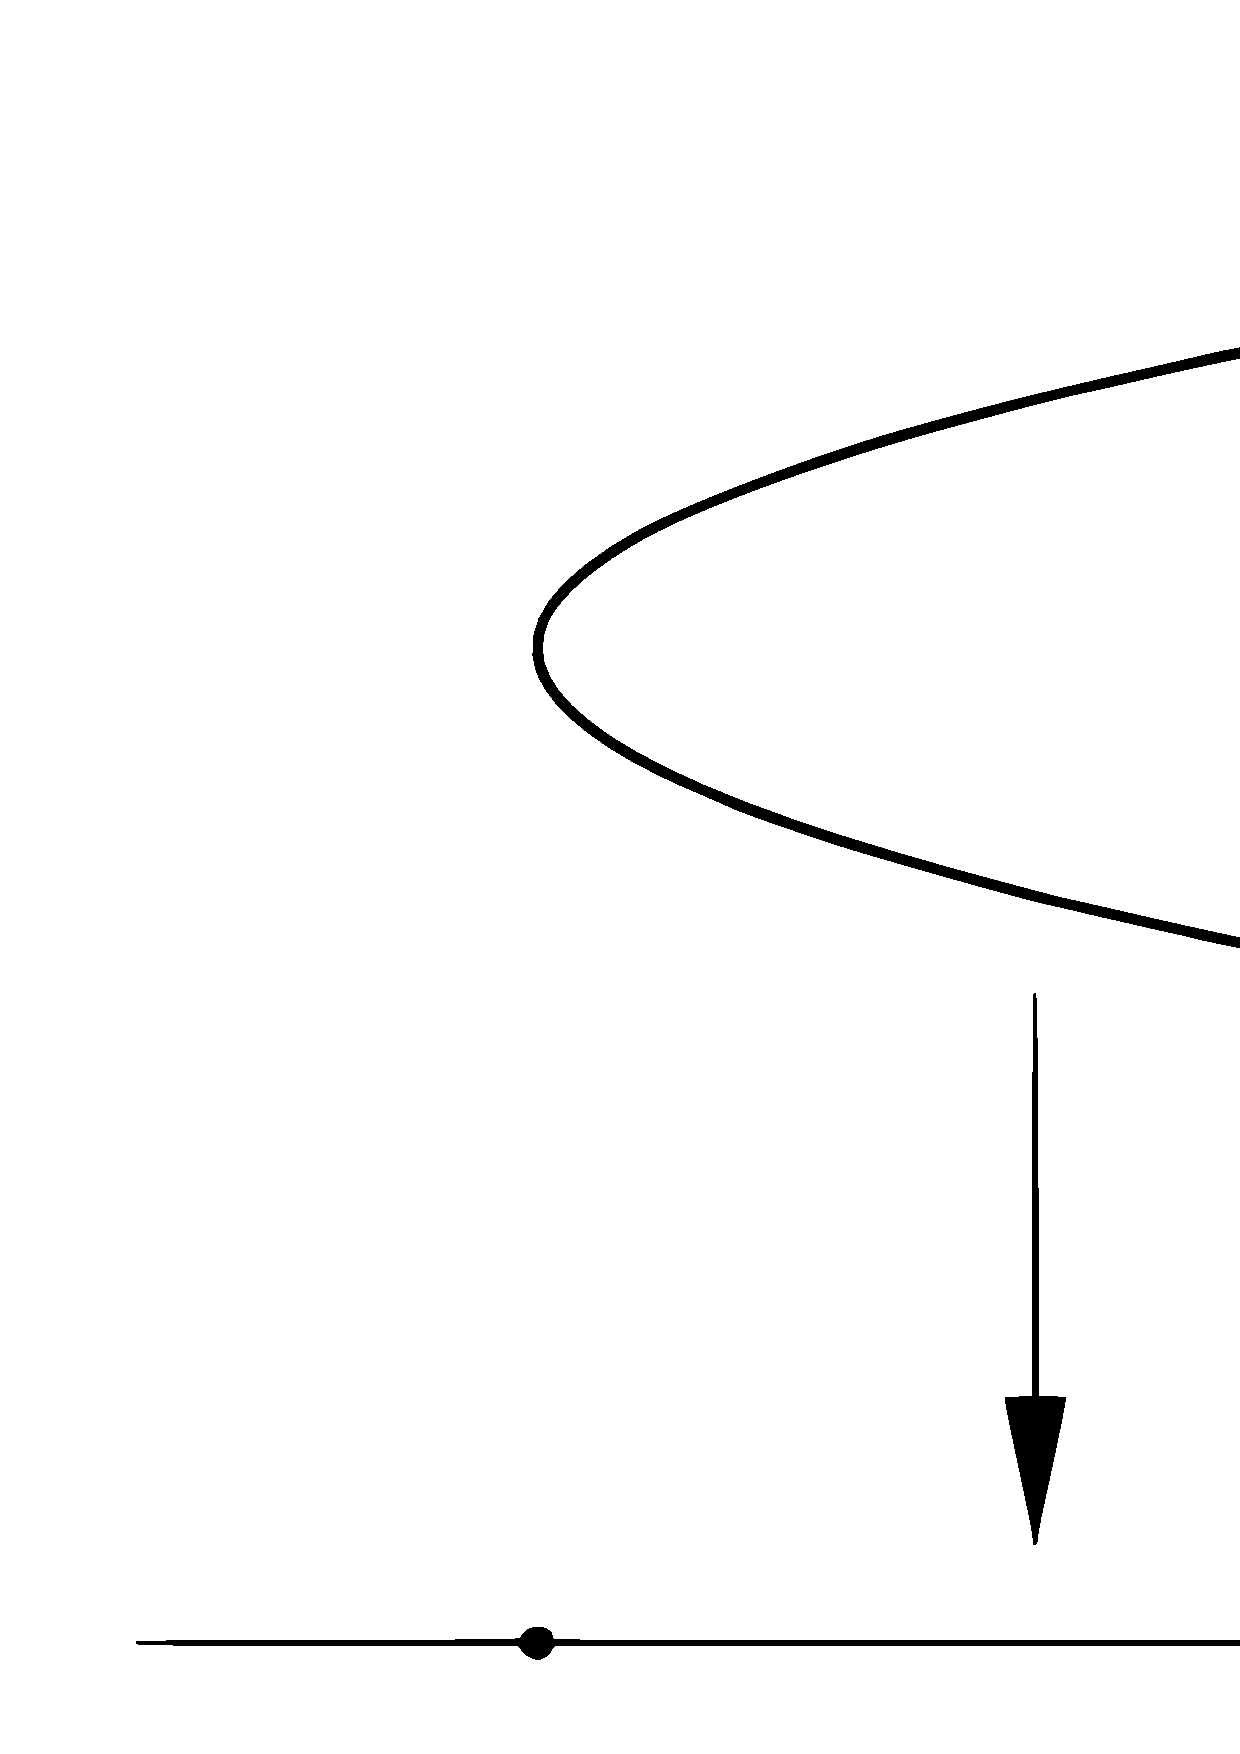
\includegraphics[scale=\scale,bb=0 0 562 68]{\PICDIR/3.png}\end{center}

在第 \ref{chap:3} 章中,我们将引入一个被称为\textit{分离性}的条件来排除$X_1$这样的概形。
\end{exe}

\paragraph*{射影空间}\addcontentsline{toc}{subsubsection}{射影空间}
黏合概形的一个重要实例是\textit{环$R$上的射影$n$-空间},记作$\P^n_R$. 他可以由$n+1$个$R$上的\textit{仿射空间}
\[
	\A_R^n=\spec R[\text{$x_1$, $\dots$, $x_n$}]
\]
黏合而成。我们将从第 \ref{chap:3} 章开始主要展开射影概形,这里我们仅用作一个黏合的展示。

这个构造与作为域上的簇的经典射影空间的构造很相似。尽管逻辑上不是必须的,但按如下工作也是方便的。首先,从$n+1$元的多项式环$R[X_0$, $\dots$, $X_n]$开集,然后取局部化
\[
	A:=R[X_0,X_0^{-1},\dots,X_n,X_n^{-1}].
\]
回忆,环$A$具有自然的\textit{分次},即一个(作为交换群的)直和分解,分解为子群$A^{(n)}$,其中$n\in \zz$,使得
\[
	A^{(n)}A^{(m)}\subset A^{(m+n)};
\]
这里$A^{(n)}$由所有$n$次单项有理分式张成。特别地,$A^{(0)}$是$A$的子环。现在取我们仿射开覆盖的环为$A^{(0)}$的$R$-子代数,第$i$个子环是包含了所有的多项式$P/X_i^{\deg(P)}$的子代数$A_i$,其中$P$是一个$R[x_0$, $\dots$, $x_n]$中的齐次元素。很清楚,$A_i$在$R$上由$n$个代数无关元
\[
	X_0/X_i,\,\dots,\,\widehat{X_i/X_i},\,\dots,\,X_n/X_i
\]
生成,其中戴帽的意思如同往常一样就是说从这列中略去这项。$A_i$于是同构于$R$上面的$n$元多项式环。此外,对$i\neq j$,作为$A$的子集,我们有
\[
	A_i[(X_j/X_i)^{-1}]=A_j[(X_i/X_j)^{-1}].
\]
它们都能被描述为所有具有$X_i^aX_j^b$形式分母的$0$次元素的子代数。如果我们取恒等映射为黏合映射,则相容性条件是显然的。

如果$X=\spec R$是一个仿射概形,我们时常用$\P^n_R$来记$\P^n_X$,并以此指代\textit{$X$上的射影空间}。因此,我们可以再一次应用黏合构造来定义\textit{任意概形$S$上的射影空间$\P_S^n$}. 这是直接的:如果$S$被仿射概形$U_\alpha=\spec R_\alpha$覆盖,我们定义射影空间$\P_S^n$为射影空间$\P_{U_\alpha}^n$沿着$U_\alpha\cap U_\beta$上的恒等映射黏起来得到的概形。
